\documentclass[a4paper]{scrreprt}

% Uncomment to optimize for double-sided printing.
% \KOMAoptions{twoside}

% Set binding correction manually, if known.
% \KOMAoptions{BCOR=2cm}

% Localization options
\usepackage[english]{babel}
\usepackage[T1]{fontenc}
\usepackage[utf8]{inputenc}

% Quotations
\usepackage{dirtytalk}

% Floats
\usepackage{float}

\usepackage{numbertabbing}

% Enhanced verbatim sections. We're mainly interested in
% \verbatiminput though.
\usepackage{verbatim}

% Automatically remove leading whitespace in lstlisting
\usepackage{lstautogobble}

% PDF-compatible landscape mode.
% Makes PDF viewers show the page rotated by 90°.
\usepackage{pdflscape}

% Advanced tables
\usepackage{array}
\usepackage{tabularx}
\usepackage{longtable}

% Fancy tablerules
\usepackage{booktabs}

% Graphics
\usepackage{graphicx}

% Current time
\usepackage[useregional=numeric]{datetime2}

% Float barriers.
% Automatically add a FloatBarrier to each \section
\usepackage[section]{placeins}

% Custom header and footer
\usepackage{fancyhdr}

\usepackage{geometry}
\usepackage{layout}

% Math tools
\usepackage{mathtools}
% Math symbols
\usepackage{amsmath,amsfonts,amssymb}
\usepackage{amsthm}
% General symbols
\usepackage{stmaryrd}

\DeclarePairedDelimiter\abs{\lvert}{\rvert}
\DeclarePairedDelimiter\floor{\lfloor}{\rfloor}

% Indistinguishable operator (three stacked tildes)
\newcommand*{\diffeo}{% 
  \mathrel{\vcenter{\offinterlineskip
  \hbox{$\sim$}\vskip-.35ex\hbox{$\sim$}\vskip-.35ex\hbox{$\sim$}}}}

% Bullet point
\newcommand{\tabitem}{~~\llap{\textbullet}~~}

\floatstyle{ruled}
\newfloat{algo}{htbp}{algo}
\floatname{algo}{Algorithm}
% For use in algorithms
\newcommand{\str}[1]{\textsc{#1}}
\newcommand{\var}[1]{\textit{#1}}
\newcommand{\op}[1]{\textsl{#1}}

\pagestyle{plain}
% \fancyhf{}
% \lhead{}
% \lfoot{}
% \rfoot{}
% 
% Source code & highlighting
\usepackage{listings}

% SI units
\usepackage[binary-units=true]{siunitx}
\DeclareSIUnit\cycles{cycles}

% Convenience commands
\newcommand{\mailsubject}{41106 - Cryptography Protocols - Series 4}
\newcommand{\maillink}[1]{\href{mailto:#1?subject=\mailsubject}
                               {#1}}

% Should use this command wherever the print date is mentioned.
\newcommand{\printdate}{\today}

\subject{41106 - Cryptographic Protocols}
\title{Series 4}

\author{Michael Senn \maillink{michael.senn@students.unibe.ch} - 16-126-880}

\date{\printdate}

% Needs to be the last command in the preamble, for one reason or
% another. 
\usepackage{hyperref}

\begin{document}
\maketitle


\setcounter{chapter}{3}

\chapter{Series 4}

\section{Textbook ElGamal in Go}

Textbook ElGamal was implemented in Go, found in the attached source code.
Completness was experimentally tested by generating random numbers $x \in
\mathbb{Z}^*_p$, and verifying that $Dec(sk, Enc(pk, x)) = x\ \forall x$.

This implementation allows messages in $\mathbb{Z}_p^*$ rather than only in the
subgroup $G$, which leaks information about the plaintexts. A secure
implementation would have to e.g. limit input values to $\mathbb{Z}_q$ and map
them to members of $G$.

\section{Additively homomorphic ElGamal encryption}

Additively homomorphic ElGamal encryption as described in the lecture was then
implemented on top of regular ElGamal. Completness was once more experimentally
tested. Random pairs of numbers $x, y < 10^4$ were generated.  It was then
verified that $\operatorname{AM-Dec}(sk, \operatorname{AM-Enc}(pk, x) \otimes
\operatorname{AM-Enc}(pk, y)) = x + y$, where $\otimes$ is the component-wise
multiplication  in $\mathbb{Z}_p^*$.

\subsection{Performance of AM-Dec}

Performance of the decryption operation was tested for two different keypairs,
with inputs in $[1, max]$ where $10^2 \leq max \leq 10^7$. Tests were done as
follows:

\begin{itemize}
		\item Two numbers $x, y \in [max / 10, max / 2]$ were generated
		\item $(R_x, C_x) := \operatorname{AM-Enc}(pk, x)$, $(R_y, C_y) :=
				\operatorname{AM-Enc}(pk, y)$
		\item $(R_z, C_z) := (R_x \cdot R_y, C_x \cdot C_y)$
		\item The duration it took for the decryption operation $z :=
				\operatorname{AM-Dec}(sk, (R_z, C_z))$ to complete was measured
		\item This duration and the order of magnitude of $z$ as
				$\floor{\log_{10}{z}}$ were logged
		\item The process was repeated multiple times and for different values
				of $max$
\end{itemize}

The resulting data was aggregated by keypair and order of magnitude, and the
mean and standard deviation of the duration calculated. Data is shown in table
\ref{tbl:performance}.

As decryption of big inputs takes exceedingly long, sample sizes for larger
inputs were chosen to be smaller.

The large standard deviations can be explained by one magnitude spanning a large
range - $9999$ and $1000$ both have magnitude $3$, yet decryption of the former
will require nearly 10 times as many computations as the later.

\begin{table}
		\begin{tabular}{llllll}
				\toprule
				$\abs{p}$ & $\abs{q}$ & Magnitude of $z$ & Avg duration & Std dev & Sample count \\
				\midrule
				1024 & 160 & 2 & \SI{7.6}{\ms}   & \SI{2.6}{\ms}   & 1000 \\
				1024 & 160 & 3 & \SI{126.5}{\ms} & \SI{46.5}{\ms}  & 1000 \\
				1024 & 160 & 4 & \SI{2.0}{\s}    & \SI{6.1}{\s}    & 200 \\
				1024 & 160 & 5 & \SI{27.2}{\s}   & \SI{72.8}{\s}   & 20 \\
				1024 & 160 & 6 & \SI{291.0}{\s}  & \SI{26.4}{\s}   & 5 \\
				2048 & 256 & 2 & \SI{22.4}{\ms}  & \SI{7.3}{\ms}   & 1000 \\
				2048 & 256 & 3 & \SI{314.2}{\ms} & \SI{97.8}{\ms}  & 1000 \\
				2048 & 256 & 4 & \SI{4.1}{\s}    & \SI{1.2}{\s}    & 200 \\
				2048 & 256 & 5 & \SI{57.1}{\s}   & \SI{15.3}{\s}   & 20 \\
				2048 & 256 & 6 & \SI{665.4}{\s}  & \SI{256.0}{\s}  & 5 \\
				\bottomrule
		\end{tabular}
		\caption{Performance of AM-Dec decrypting plaintexts $z$ of differnt dimensions}
		\label{tbl:performance}
\end{table}

Figure \ref{fig:performance} visualizes this data in a logarithmic plot. It
clearly shows that generally processing time grows exponentially with the
magnitude of the input. This matches expectations as, for an input of magnitude
$k$, $O(10^k)$ possible exponents need to be tried in the decryption process.

% TODO sentence
The figure also shows that different key parameters cause a linear difference
in processing time. This matches with the expectation that the performance of
efficient modular exponentiation is linear in the bit length of its parameters.
Indeed the difference in decryption times approaches two, matching the
difference of two in the bit length of the modulus.

\begin{figure}[h]
        \centering
		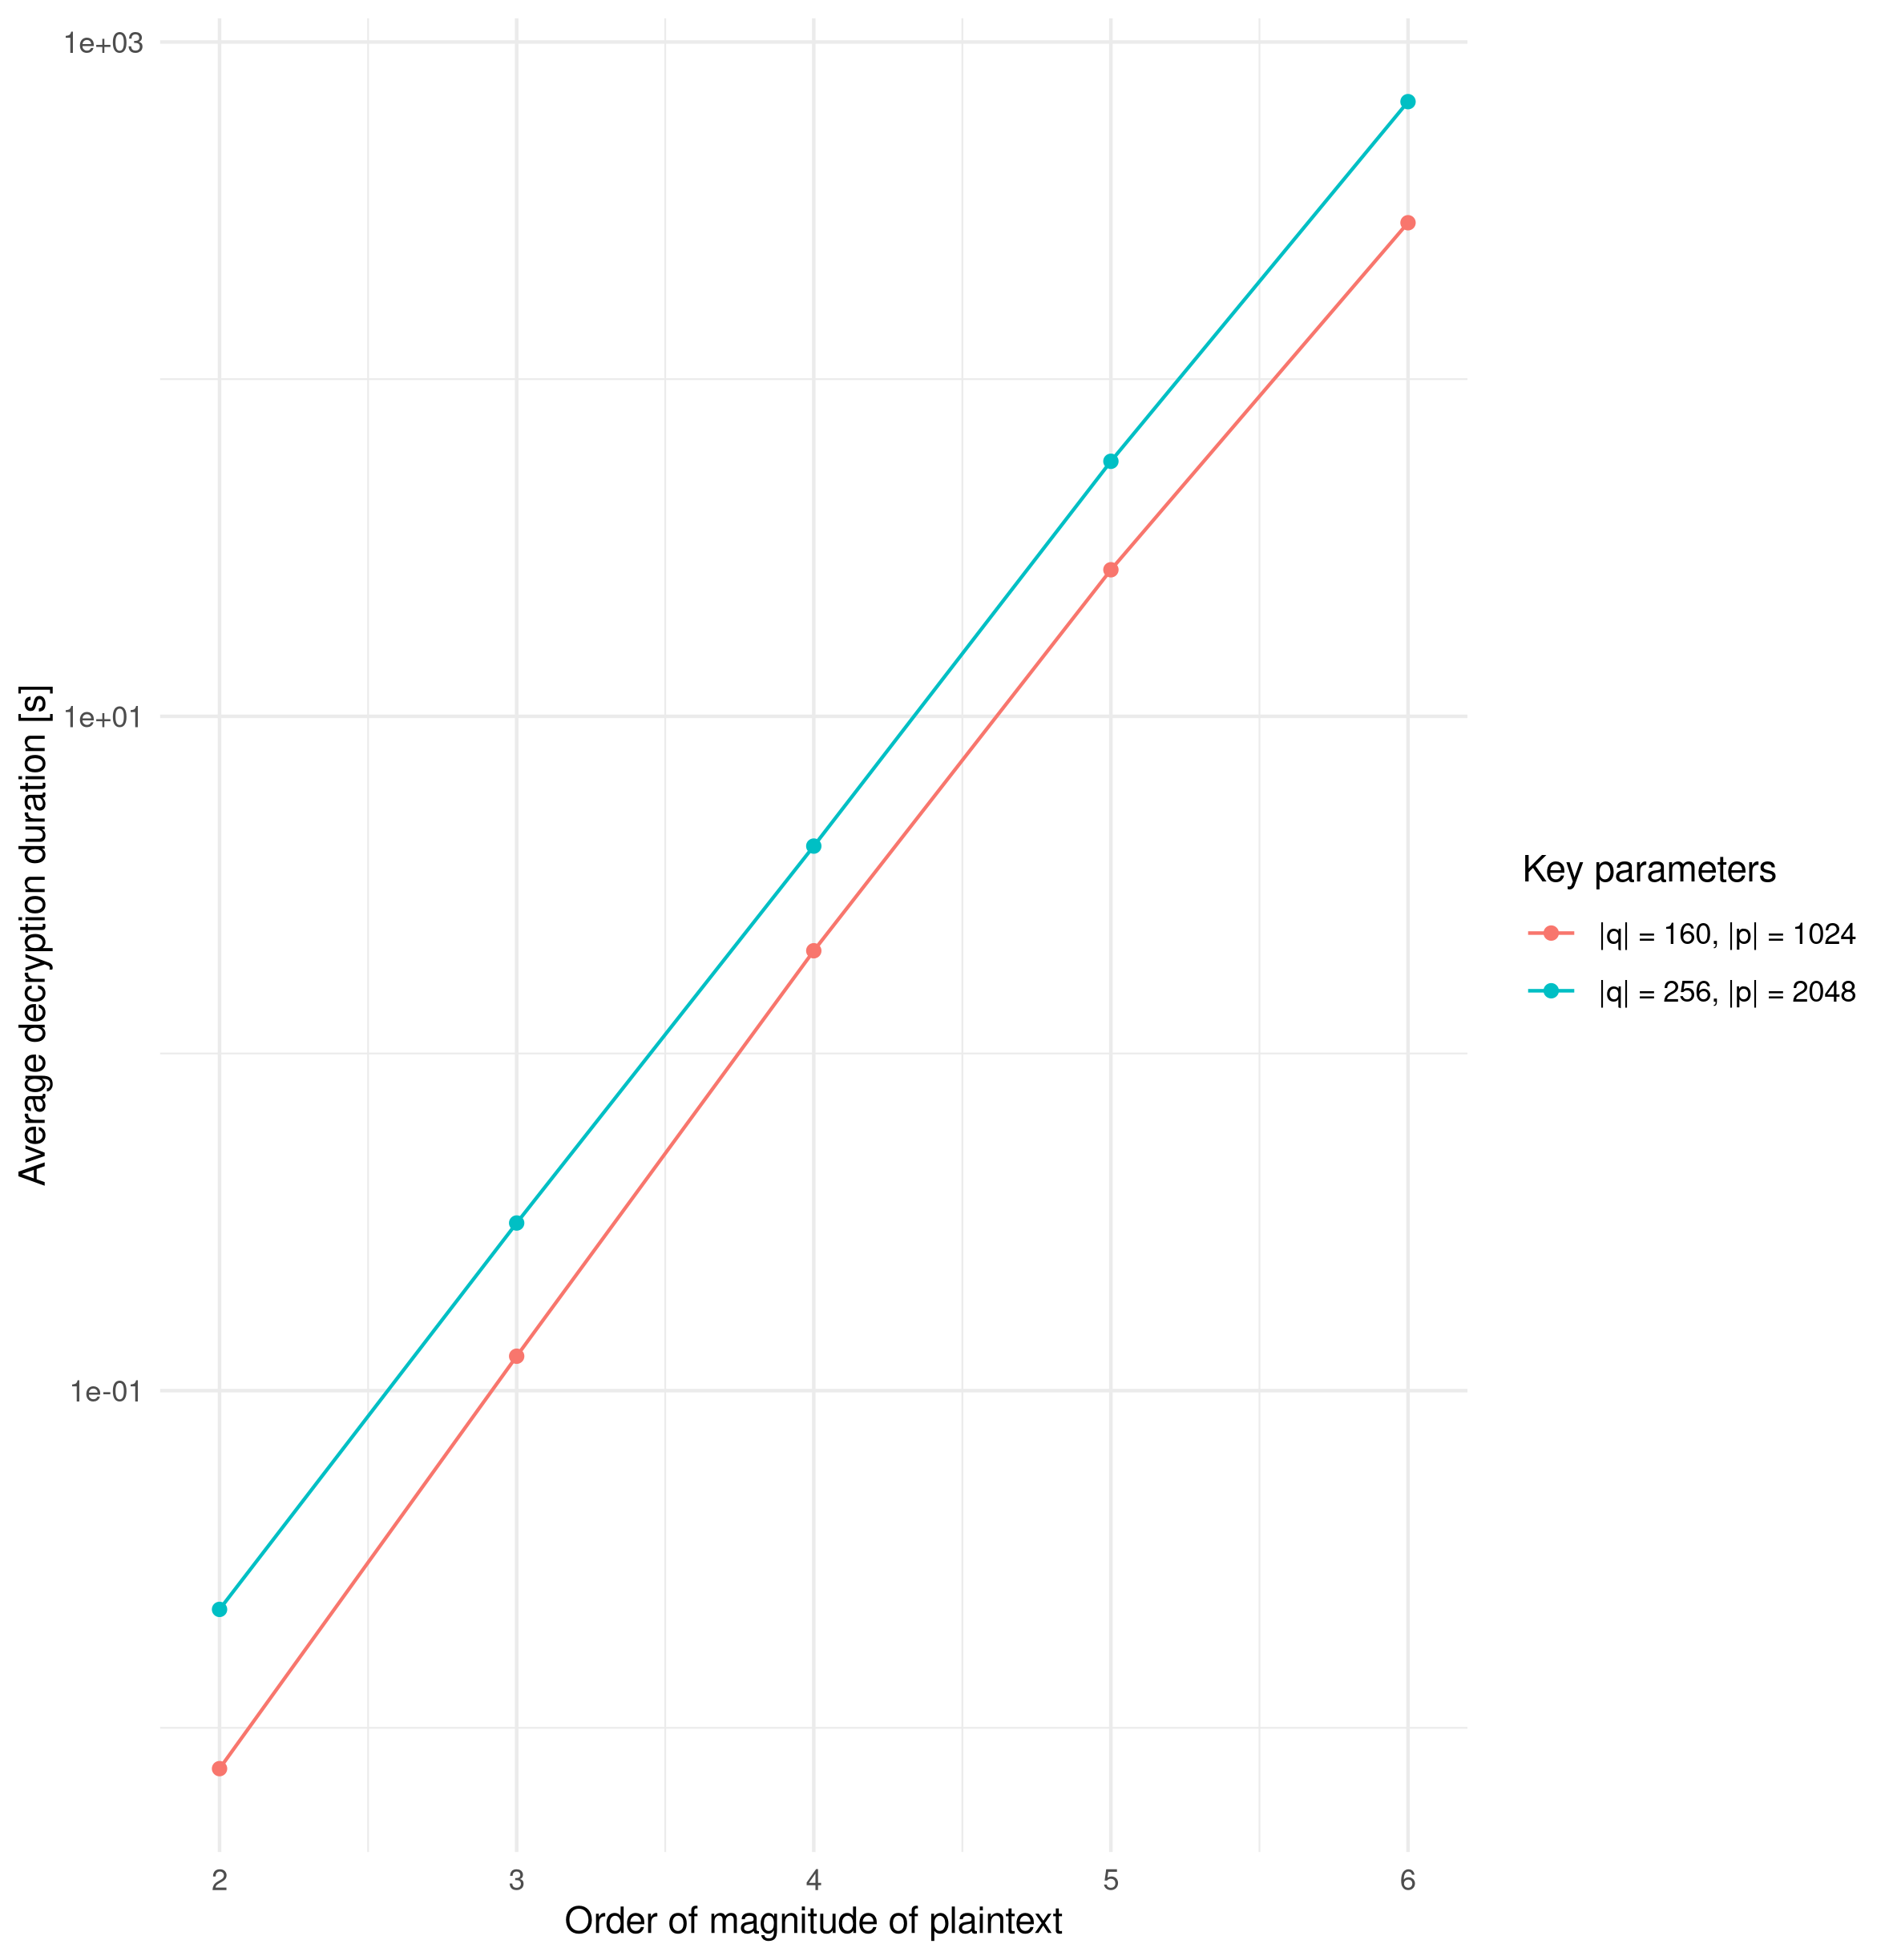
\includegraphics[width=\textwidth]{elgamal_performance}
		\caption{Performance of decryption in additively homomorphic ElGamal}
		\label{fig:performance}
\end{figure}

\subsection{Improving performance of additively homomorphic ElGamal cryptosystem}

One natural way to optimize performance of the additively homomorphic ElGamal
cryptosystem is to parallelize the brute-force search in the decryption
function. For any non-trivial message space $[1, max]$ this search quickly uses
up the vast majority of processing time.

Recall that this brute-force search has the goal of finding an $i$ such that
$g^i \equiv h \pmod{p}$, which is done by iterating through permissible values
of $i \in [1, max]$. The iterations of the loop are independent of each other,
requiring only read-only access to a shared value of $h$. This allows easily
dividing the iterations between different processes, leading to a linear
speedup with the number of parallel running processes.

An additional approach to optimizing this cryptosystem is to optimize
performance of the underlying modular exponentation. If the generator $g$ can
be chosen as a power of two for example, multiplication turns into a bit shift.

\end{document}
